\documentclass[english]{tktltiki2}

% -- Packages --

\usepackage[utf8]{inputenc}
\usepackage[T1]{fontenc}
\usepackage{lmodern}
\usepackage{microtype}
\usepackage{amsfonts,amsmath,amssymb,amsthm,booktabs,color,enumitem,graphicx}
\usepackage[pdftex,hidelinks]{hyperref}

% Automatically set the PDF metadata fields
\makeatletter
\AtBeginDocument{\hypersetup{pdftitle = {\@title}, pdfauthor = {\@author}}}
\makeatother

% -- Language --

\usepackage[fixlanguage]{babelbib}

% Add bibliography to the table of contents
\usepackage[nottoc]{tocbibind}

% -- tktltiki2 options --

\title{Advances in Streamlining Software Delivery on the Web and its Relations to Embedded Systems}
\author{Kasper Hirvikoski}
\date{\today}
\level{Master’s thesis}
\abstract{Abstract.}

\keywords{keyword}
\classification{}

\begin{document}

% -- Front matter --

\frontmatter

\maketitle
\setcounter{page}{2}
\makeabstract

\tableofcontents

% -- Main matter --

\mainmatter

% -- Introduction --

\section{Introduction}

Software delivery on the web has over the years evolved into a rather established process. A software is developed iteratively through multiple stages, which ensure the user’s requirements and the quality of the product or service. These stages form what is called the deployment pipeline~\cite{Fow06, HF11, Fow13a, Fow13b}.

The deployment pipeline nowadays usually consists of at least three stages: development, staging and production. Organisations alter these stages depending on their size and needs. Using modern iterative and incremental processes, a software is developed feature-by-feature by iterating through these stages. Development starts in the development stage where developers build the feature requested by the customer or user. The feature is then tested in the staging phase, which represents the production setting. When the feature has been validated, it is then deployed to production. If necessary, each stage can be repeated until the feature is accepted. The stages are short and features are deployed frequently — in some cases even multiple times a day~\cite{OR11, Sny13, Rub14}.

Software engineering consists of various different processes and practises for ensuring the quality of the product or service — nowadays more or less based on Agile and Lean ideologies and practises~\cite{BBB01a, Fow05, Mon12}. At the low level, developers use source code management to keep track of changes to the software and to collaborate with other team members. To reinforce that the features work as intended, developers write automated test cases. Teams can also use more social methods — such as reviewing each other’s code — to validate the implementations. These practises form the basis for Continuous Integration and Continuous Deployment~\cite{Fow06, HF11, Fow13a, Fow13b}. Software changes are frequently integrated, tested and deployed — automatically in each stage. The first two form Continuous Integration and the latter Continuous Deployment. If any stage fails, the process starts from the beginning.

The web enables the use of the deployment pipeline and its practises in an unprecedented way~\cite{KLS09}. Due to the distributed nature of the web, software can be deployed as needed and the user always sees the newest version without the need of any interaction. This eases the use of many cutting-edge methods~\cite{KLS09}. Deploying software as needed has allowed developers to experiment with different implementations of a feature. These changes can target anything from a more optimised algorithm to something more user-faced, such as improvements to the user experience of a product~\cite{KLS09}. These practises have started to formalise as Continuous Experimentation~\cite{FGM14}.

Not all software can be developed easily this way. Many embedded systems, which have a dedicated function within a larger mechanical or electrical system, require hardware to accompany the software. This presents a variety of challenges to overcome. Hardware can require thorough planning and iterating can take time. Contexts such as cross-platform support, robotics, aerospace and other embedded systems pose interesting cases. Many of these contexts can at a glance seem regarded as models for more traditional sequential software engineering processes with heavy planning, documentation and long development phases. However, even NASA’s earlier missions have iterated on the successes and failures of previous ones. Even though it can be more difficult, hardware can be build and tested iteratively with new approaches such as prototyping and 3D-printing.

This raises an interesting research topic — \emph{presenting the advances in streamlining software delivery on the web and relating its practises and their advantages and challenges to embedded systems}. Using case studies to identify which practises are used, how they could be improved and how new practises could be incorporated to these settings.

The approach of my thesis is to identify how modern software development methods, such as Agile and Lean, suit embedded settings and if and how they have been adapted to these environments. Moreover, the aim is to identify which modern Continuous Integration, Delivery and Experimentation practises are used, how they could be improved and how new practises could be incorporated to more embedded settings. Can we determine how they compare to web practises?

The hypothesis is that there should be no reason why these practises could not be successfully used and cleverly adapted to hardware settings.

My research method for this thesis was reviewing the current practises in literature and industry. I also conducted several interviews with the industry working on leading embedded systems to get a view on if and how the deployment pipeline has changed the development of hardware related products.

% -- Software Delivery --

\section{Software Delivery}

Software development has changed notably in the past few decades. Going back, it was not until 1968, when the term software engineering was introduced by the NATO Science Committee~\cite{NR69}. By that time, it was considered that software development had drifted into a crisis, where a wider gap was forming between the objectives and end-results of software projects. Additionally, it was getting increasingly difficult to plan the cost of development. A collective effort was put in place to establish a more formalised method for software development — similar to traditional engineering. It was considered necessary that the foundation for delivering software should be more theoretical with laid principles and practises~\cite{NR69}. By 1969, the term software engineering had become well-established~\cite{BR70}.

Software development processes began to form. Notably in 1970, Winston W. Royce published a paper that described a formal approach for sequentially developing a software based on previously used practises~\cite{Roy70}. It was only later named as the waterfall model~\cite{Boe88, LB03}. The process consists of multiple stages that should be carried after the previous has been reviewed and verified. See figure~\ref{figure:waterfall-model}. It begins by mapping the requirements for the entire software, then proceeding to designing the architecture, followed by implementing the plan, verifying the result is according to the set requirements, and finally maintaining the product~\cite{Roy70}. Each stage is planned and documented thoroughly. However, contrary to what has been referred, Royce presented the model as a flawed, non-working model~\cite{Roy70}. If any of the stages fail, serious reconsideration of the plan or implementation might be necessary. Therefore sequentially following the stages would not produce what was intended and inevitably previous stages would need to be revisited~\cite{Roy70}. Nevertheless, this was overlooked and the waterfall model became the dominant software development process for software standards in government and industry for the time-being~\cite{Boe88, LB03}.

\begin{figure}[h!]

    \vspace{1cm}
    \centering

    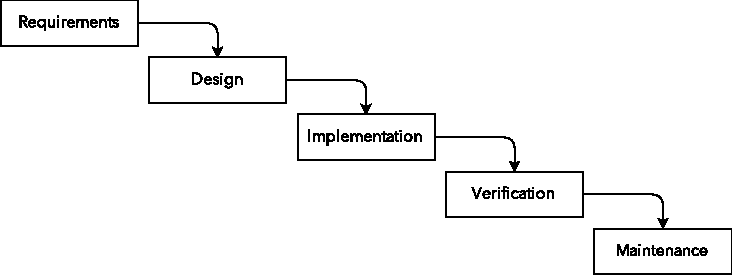
\includegraphics{waterfall-model}

    \caption{Waterfall Model}
    \label{figure:waterfall-model}

    \vspace{1cm}

\end{figure}

Waterfall-oriented models are considered heavy. The waterfall model has been criticised as too controlled and managed, documentation-oriented and over-incremental~\cite{Boe88, LB03}. More lightweight iterative processes were proposed as opponents for incremental software development in the later part of the nineteen hundreds~\cite{LB03}. In fact, early applications of iterative and incremental development dates as far back as the mid-1950s~\cite{LB03}. Fast-forward to 2001, when a group of software developers met to discuss new lightweight development principles. As the result of these discussions, a manifesto for Agile software development was published~\cite{BBB01a}. Four principles were proposed for Agile software development: focusing on individuals and interactions over processes and tools, focusing on working software over comprehensive documentation, focusing on customer collaboration over contract negotiation and responding to change over following a plan. The manifesto does not dismiss the value of the latter, but considers the former more valuable~\cite{BBB01a}. Iterative processes started to gain mainstream traction~\cite{LB03}. Software development was considered as an ongoing process, where a product should be build in small increments, iteratively going through the development stages. Instead of planning, designing and implementing the whole software, the software should be build iteratively by repeating all of these steps in shorter more manageable parts. See figure~\ref{figure:iterative-development}. Hence, any issue or miss-communication could be discovered early and fixed accordingly.

\begin{figure}[h!]

    \vspace{1cm}
    \centering

    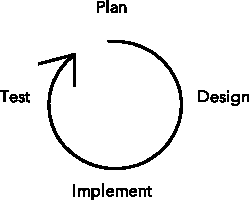
\includegraphics{iterative-development}

    \caption{Iterative Development}
    \label{figure:iterative-development}

\end{figure}

\subsection{Adapting to Requirements}

The demands for software products are continuously shifting. It is not always obvious what the users want. In some cases, users do not know what they are looking for, until you show them what they need. An average client has little knowledge on how software products work or how they are built. Therefor, it is exceedingly difficult for a client to map specifically what they require from a software product. In most cases, rigorously planning a software beforehand will not work. Agile development tries to create a framework, where processes and practises can take these requirements into consideration.

Prominently, being “agile” means effectively responding to change. These course corrections are rapid and adaptive. The highest priority is to satisfy the customer trough continuously delivering valuable software from early on~\cite{BBB01b}. Software should be delivered frequently in short increments. These increments, also referred as iterations in Agile development, should take no more than a couple of weeks to a couple of months — the shorter the better. Throughout the project, teams respond to change by having effective communication among all stakeholders for the product daily. The best means for conveying information is face-to-face conversation~\cite{BBB01b}. A stakeholder represents the views for the users or clients. By taking the stakeholders as part of the team, developers can react when something is not working as intended. Studies show that developers see the ongoing presence of stakeholders helpful for development~\cite{DD08}. An Agile process is driven by the customers descriptions of what is required~\cite{BBB01b}. These requirements may be short-lived and that must be kept in focus. Changes are unavoidable. Users’ desires evolve and this must be harnessed to the customer’s competitive advantage~\cite{BBB01b}. It is not uncommon for requirements to change even late in development.

One key premiss for Agile development is to reduce the burden of the process. Working software is the primary measure of progress~\cite{BBB01b}. A process should not hinder the work of a team — on the contrary it should permit the team to function to its full extent. By organising the team to be in control of the process, the framework facilitates rapid and incremental delivery of software. Projects should be based on motivated individuals~\cite{BBB01b}. Motivation is maintained by creating a constructive environment and giving the necessary support when needed. Trusting the team is of the utmost importance~\cite{BBB01b}.

\subsection{Ensuring Quality}

Assuring quality is not an easy task. ISO 9000-standard defines quality as the extent of how well the characteristics of a product or service fulfil all of the requirements, the needs and expectations, set by the stakeholders~\cite{ISO9000}. IEEE defines software quality as the degree to which a system, component or process meets the specified requirements as well as the customer’s and user’s needs or expectations~\cite{IEEE1074}. Both definitions focus strongly on fulfilling the user’s needs.

Software development is challenging. Users perceive quality as working software, but most of all emphasising good technical design and implementation makes the development process easier. People, time and money are limiting factors for ensuring quality. Strict deadlines and scarce resources have direct effects. Furthermore, human factors play a considerable role. Several empirical studies reinforce the significance of Agile development processes and practises as improving quality in software~\cite{SS10}. Evidently being “agile” should in the long term make development more predictable and eventually lead to shorter development times and minimised costs. This provides an environment for being adaptive.

In addition to focusing on satisfying the customers needs, Agile development promotes continuous attention on technical excellence and good design practises~\cite{BBB01b}. Even so, this should not be accomplished by hindering simplicity. Simplicity maximises the amount of work that can be accomplished. The Agile Manifesto states that the best architectures, requirements and designs emerge from self-organising teams~\cite{BBB01b}. After regular intervals, the team members reflect on how they have performed and how they can become more effective. This is how the team can then tune and adjust its behaviour appropriately.

\subsection{Processes and Practises}

Processes and practises assist the development process. They create the framework and guidelines within a team can develop a suitable environment to deliver software~\cite{Kni07}. They also help to maintain quality. Modern development strongly focuses on Agile and Lean ideologies and practises~\cite{BBB01a, Fow05, Mon12}.

At the low level, developers use source code management to keep track of changes to the software and to collaborate with other team members. Source code management enables multiple developers to work on a single project, while also creating a history for the entire project. When a problem arises, developers can go back in time to look at the source code at any given point in time. To ensure features work as intended, developers use automated test cases to verify expected behaviour. There is a clear correlation between higher test coverage resulting in fewer errors in software~\cite{MND09}. Tested code has a better change of detecting errors than untested code. Teams can also use more social methods — such as reviewing each other’s code — to validate the implementations. Pair programming, coding dojos and hackathons provide tools for improving skills and solving complex problems together.

Agile development only provides a framework for software delivery. It does not specify concretely how development should be organised. Most notably, Scrum and Extreme Programming (XP) have created a structure for Agile development~\cite{LB03, SS10}. Scrum provides a framework for managing development. It focuses on how development should be planned, managed and scheduled. It does not provide any strict practises, instead it gives guidelines for how customer requirements should be discovered, prioritised, and how the development of these features is split into iterations.

Scrum has been strengthened with practises such as test-driven development (TDD) and pair programming. These are defined in XP. In test-driven development, features are developed by writing the expectations for a feature as tests before actually implementing the code. In pair programming, developers develop features in pairs.

\subsection{From Agile to Lean}

As time has elapsed, developers have simplified software delivery even more. Agile has turned into Lean. Being “lean” means reducing the amount of “waste” around software development. Iterations have turned into building single features at a time. Instead of building a frame for a car, a development process should essentially start with building a bicycle first. To evaluate an idea, developers should begin by developing a minimum viable product (MVP) to validate the implementation has value. Being “adaptive”, has transformed into quantitatively assessing what effects changes have. This build-measure-learn cycle has transformed how features are developed and validated. See figure~\ref{figure:build-measure-learn}.

\begin{figure}[h!]

    \vspace{1cm}
    \centering

    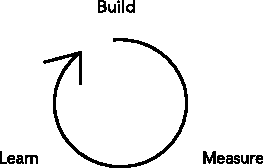
\includegraphics{build-measure-learn}

    \caption{Build-Measure-Learn Cycle}
    \label{figure:build-measure-learn}

\end{figure}

% -- Deployment Pipeline --

\section{Deployment Pipeline}

Deployment pipeline.

\subsection{Development}

Development.

\subsection{Staging}

Staging.

\subsection{Production}

Production.

% -- Using Web as a Platform --

\section{Using Web as a Platform}

Using Web as a platform.

\subsection{Continuous Integration}

Continuous Integration.

\subsection{Continuous Deployment}

Continuous Deployment.

\subsection{Continuous Experimentation}

Continuous Experimentation.

% -- Towards Embedded Systems --

\section{Towards Embedded Systems}

Towards embedded systems.

\subsection{Using Hardware as a Platform}

Using hardware as a platform.

\subsection{Adapting for Deployment Pipeline}

Adapting for deployment pipeline.

% -- Example Case --

\section{Example Case}

Example case.

% -- Conclusions --

\section{Conclusions}

Conclusions.

% -- References --

\bibliographystyle{babalpha-lf}
\bibliography{references}

\end{document}
